\section{Algorithm and Process Flow Specifications}
\label{appendix:algorithm}
% Retains the original section label so every \ref{sec:system_sm2} elsewhere in
% the report now resolves to this appendix rather than breaking.
\label{sec:system_sm2}

This appendix carries the specification of the spaced-repetition scheduling
model, which the body of the report states only in summary, together with the
flow diagrams for those processes whose control flow is difficult to follow
from prose alone. A flow earns a diagram here on one criterion: that its shape
is unusual enough that a linear description of it misleads. Each of the seven
crosses several processes, branches on conditions that are not obvious from the
endpoint that starts it, and has at least one path that exists only to handle a
failure or an attempt at abuse. The diagrams show the branches and the failure
paths together, which prose in sequence cannot. They are ordered as the system
is exercised rather than as the packages are named: the learner's own loop
first, then the authoring pipelines that fill it, then the assessment those
pipelines produce, and finally the pathway structure above all of them.

\subsection*{Spaced repetition: why this is an appendix}

The scheduling model below governs how aBridgeAI decides when a learner sees a
card again. It is specified here rather than in the body of the report
because the present iteration does not evaluate it: establishing that a
scheduling policy improves retention requires a longitudinal cohort study that
this project's timeline does not accommodate, and reporting a design as a
contribution without evidence for it would overstate what has been shown. What
the system does implement is described in Section~\ref{sec:impl_sr}; what
follows is the specification that implementation realises, retained in full so
that the algorithm is reproducible and available for evaluation in later work.

\subsection{Hybrid SM-2 and Q Derivation}
\label{sec:q_derivation}
aBridgeAI adopts SM-2 as the scheduling foundation for quiz-based SR, extending it with two modifications: replacement of self-reported $Q$ with an algorithmically derived value grounded in objective response signals, and introduction of a calibration weight that dampens early EF growth until sufficient retrieval evidence has accumulated. The theoretical motivation for these departures is established in Section~\ref{sec:sm2_limitation}; this section specifies their formal implementation.

\paragraph{Teacher-Defined Expected Response Time}
Each quiz card carries a teacher-assigned expected response time $T_{\text{exp}}$, set explicitly during the card review phase before publication. This value reflects the teacher's domain judgment of the duration within which a student demonstrating confident, independent recall should be able to answer the question. $T_{\text{exp}}$ is a mandatory field — no card may be published without it — and may be revised by the teacher at any point prior to or during deployment. Because $T_{\text{exp}}$ is teacher-defined rather than formula-derived, it incorporates contextual knowledge of the question's cognitive demand that no surface-feature heuristic could reliably approximate: a teacher setting $T_{\text{exp}}$ for a TCP troubleshooting question draws on their understanding of how long a competent student requires to reason through the problem, not merely how long the question takes to read.

\paragraph{Time Ratio}
Each student response is normalised against the card's expected response time via a dimensionless time ratio $\rho$:

\begin{equation}
    \rho = \frac{T_{\text{actual}}}{T_{\text{exp}}},
\end{equation}



where $T_{\text{actual}}$ is the elapsed time in milliseconds between question presentation and answer submission. A value of $\rho < 1$ indicates the student responded faster than expected; $\rho = 1$ indicates exact correspondence with the teacher's expectation; and $\rho > 1$ indicates the response exceeded the expected window. Because $\rho$ is dimensionless and normalised against a card-specific baseline, it is comparable across questions of differing complexity — a student answering a hard question in exactly the expected time produces the same $\rho$ as a student answering an easy question in its expected time.

\paragraph{Q Value Assignment}
The quality response value $Q \in \{0, 1, 2, 3, 4, 5\}$ is determined by two signals in sequence: first, whether the answer was correct; second, for correct answers, whether a hint was used. Within each branch, $Q$ is resolved as a continuous function of $\rho$ rather than through fixed threshold boundaries, ensuring that the mapping from response latency to recall quality varies smoothly with the ratio rather than producing discontinuous jumps at arbitrary cutoff values.

An incorrect answer yields $Q = 0$ unconditionally, reflecting the position established in Section~\ref{sec:sm2_limitation} that partial credit for failed recall creates an advancement pathway inconsistent with competency-based progression.

For correct answers where a hint was used, the student has demonstrated assisted rather than independent recall. The ceiling is therefore $Q = 2$, with the value resolved by:

\begin{equation}
Q = \max\!\left(1,\ 
    2 - \left\lfloor \rho \right\rfloor
\right), \quad Q \in \{1, 2\}.
\end{equation}

This maps $\rho < 1$ and $\rho \in [1, 2)$ to $Q = 2$, and $\rho \geq 2$ — indicating the student took more than twice the expected time even with a hint — to $Q = 1$. No hint usage can produce $Q \geq 3$, preserving the SM-2 convention that scores of 3 and above require independent retrieval \cite{wozniak1998sm2}.

For correct answers where no hint was used, $Q$ is mapped from $\rho$ over the range $\{3, 4, 5\}$ as:

\begin{equation}
Q = \max\!\left(3,\ 
    5 - \left\lfloor 2\rho \right\rfloor
\right), \quad Q \in \{3, 4, 5\}.
\end{equation}

This assigns $Q = 5$ when $\rho < 0.5$ — the student answered in less than half the teacher's expected time, consistent with effortless retrieval; $Q = 4$ when $0.5 \leq \rho < 1$ — the student answered within the expected window, consistent with controlled but fluent recall; and $Q = 3$ when $\rho \geq 1$ — the student exceeded the expected time, consistent with laboured reconstruction despite eventual correctness \cite{benjamin1996}. The floor of 3 ensures that any independent correct response, regardless of latency, is treated as a passing recall event and does not trigger an interval reset. The complete assignment rule is summarised in Table~\ref{tab:q_assignment}.

\begin{table}[H]
\centering
\small
\renewcommand{\arraystretch}{1.3}
\caption{Q value assignment rules based on correctness, hint usage, and time ratio $\rho$. Boundaries at $\rho = 1$ and $\rho = 2$ correspond to the teacher-defined expected response time and twice that value respectively; the boundary at $\rho = 0.5$ corresponds to half the expected time.}
\begin{tabular}{|l|l|c|l|}
\hline
\textbf{Correctness} & \textbf{Hint Used} & 
\textbf{Time Ratio $\rho$} & \textbf{$Q$} \\
\hline
Incorrect & — & any & 0 \\
\hline
Correct & Yes & $\rho \geq 2$ & 1 \\
Correct & Yes & $\rho < 2$    & 2 \\
\hline
Correct & No  & $\rho \geq 1$ & 3 \\
Correct & No  & $0.5 \leq \rho < 1$ & 4 \\
Correct & No  & $\rho < 0.5$  & 5 \\
\hline
\end{tabular}
\label{tab:q_assignment}
\end{table}

The boundaries in the no-hint branch — $\rho = 1$ and $\rho = 0.5$ — require no external calibration because they derive directly from the teacher-defined $T_{\text{exp}}$: $\rho = 1$ is exactly the teacher's competency expectation, and $\rho = 0.5$ is half of it. Similarly, the hint branch boundary at $\rho = 2$ represents twice the expected time, a duration at which continued difficulty despite hint exposure reasonably indicates weak encoding rather than momentary hesitation. All boundaries are therefore interpretable as multiples of $T_{\text{exp}}$ rather than as independently chosen constants, and their justification is grounded in the semantics of the teacher-defined baseline rather than in arbitrary numerical choices.

\paragraph{EF Update and Interval Scheduling}
The derived $Q$ value is passed into the standard SM-2 EF 
update rule:

\begin{equation}
EF_{\text{new}} = EF_{\text{old}} + 
\left(0.1 - (5 - Q)\left(0.08 + (5 - Q) \cdot 
0.02\right)\right),
\end{equation}

with $EF$ bounded below by $EF_{\min} = 1.3$. The review 
interval follows the standard SM-2 recurrence:

\begin{equation}
I(n) =
\begin{cases}
1               & \text{if } n = 1 \\
6               & \text{if } n = 2 \\
I(n-1) \cdot EF & \text{if } n > 2,
\end{cases}
\end{equation}

where $n$ denotes the repetition count. If $Q < 3$, the item is considered failed: $I$ resets to 1 day and $n$ returns to zero regardless of prior history. The EF penalty is applied before the reset, ensuring that repeated failures progressively reduce the interval growth rate even as the absolute interval restarts.

\paragraph{Interval Jitter}
To prevent review storms caused by the simultaneous scheduling of multiple cards to the same date, a jitter factor $\varepsilon \sim \mathcal{U}(-0.1,\ 0.1)$ is applied multiplicatively to each computed interval:

\begin{equation}
I_{\text{final}} = I(n) \cdot (1 + \varepsilon).
\end{equation}

The magnitude of $\varepsilon$ is small enough to have negligible effect on retention outcomes while distributing scheduled reviews across a window of approximately $\pm 10\%$ of the nominal interval, preventing the concentration of review obligations on single calendar dates.

\paragraph{Interval Ceiling and Card Retirement}
As established in Section~\ref{sec:sm2_limitation}, the SM-2 recurrence is unbounded above. aBridgeAI bounds it with an organisation-configurable ceiling $I_{\max}$ applied after jitter, so that the ceiling is a true upper bound rather than one the jitter may exceed:

\begin{equation}
I_{\text{scheduled}} = \min\left(I(n) \cdot (1 + \varepsilon),\ I_{\max}\right).
\end{equation}

The default $I_{\max} = 36500$ days is adopted from Anki, where the equivalent setting carries the same default, and at that value the ceiling does not bind: the longest interval reachable through eight consecutive maximal-$EF$ reviews is approximately $1465$ days. The direction of the control is worth stating explicitly, because it is counter-intuitive. Lowering $I_{\max}$ does not reduce review load; it guarantees that no item drifts out of sight for longer than the configured period, and therefore \textit{increases} the number of reviews a student is asked to perform. It is a retention floor, not a workload ceiling.

A second, independent parameter converts that bound into a terminal state. When card retirement is enabled and a review earns an interval exceeding $I_{\max}$, the card ceases to be scheduled: it retains its $EF$, its interval, its repetition count and its full review history, but holds no next due date and is therefore absent from every due-card read. Retirement requires the computed interval to exceed $I_{\max}$ strictly, so an installation may set the ceiling to the cadence at which it wishes items to settle without that cadence itself triggering retirement.

Retirement is terminal in both directions. A subsequent encounter with the item --- in a later quiz, for instance --- is graded and recorded as a review, because the retrieval did occur, but does not return the card to the queue; and a failed review neither retires a card nor revives a retired one, since the reset to a one-day interval addresses an item still being consolidated rather than one already released.

This parameter is disabled by default, and the reason is theoretical rather than operational. Under the Two-Component Model described in Section~\ref{sec:sm2_limitation}, retrievability decays continuously between reviews for every item regardless of its stability; no state exists in which an item is no longer subject to forgetting. A retirement point therefore cannot be justified as a claim about memory. It is justified instead as a bounded-scope decision: where the material belongs to a course of finite duration, an institution may reasonably decide that review obligations should not outlive the enrolment that created them. The distinction matters for interpretation of the resulting data --- a retired card records that scheduling stopped, not that the item was permanently learned.

\paragraph{Calibration Weight}
SM-2 initialises $EF$ at $2.5$ for all items, implicitly assuming average retention ability from the first review. In an institutional context where EF influences lesson unlock eligibility, an overestimated early EF produces intervals that grow too quickly before the algorithm has accumulated sufficient evidence of the student's retention capacity for that item. To address this, aBridgeAI applies a calibration weight $\alpha$ to positive EF increments during the first three repetitions of any card:

\begin{equation}
EF_{\text{new}} = 
\begin{cases}
EF_{\text{old}} + \alpha \cdot \Delta EF 
  & \text{if } n \leq 3 \text{ and } \Delta EF > 0 \\
EF_{\text{old}} + \Delta EF 
  & \text{otherwise},
\end{cases}
\end{equation}

where $\Delta EF$ denotes the increment produced by the standard update rule and $\alpha = 0.6$. Negative increments — produced when $Q < 4$ — are applied at full magnitude regardless of $n$, ensuring that evidence of forgetting is incorporated immediately while evidence of retention accumulates more conservatively. Once $n > 3$, $\alpha = 1$ and the standard update rule applies without modification. This asymmetric initialisation ensures faster convergence onto the student's true retention profile than an optimistic starting assumption would permit, consistent with the principle that conservative initial models require fewer corrective cycles than overconfident ones \cite{wozniak1998sm2}.

\subsection{Individualised Learner Modeling}
\label{sec:individualised_modeling}
A foundational design decision in aBridgeAI is the isolation of all SM-2 state variables at the level of the student-card pair rather than the card itself. The Easiness Factor $EF$, review interval $I$, repetition counter $n$, and next scheduled due date are maintained as independent records for each unique combination of student and knowledge item. Two students reviewing the same card therefore accumulate entirely separate $EF$ trajectories reflecting their individual retrieval histories, and no student's scheduling is influenced by the aggregate performance of peers on shared material. This isolation is a theoretical necessity as much as an implementation choice: the same observable response pattern may reflect different underlying knowledge states in different learners depending on prior experience, domain familiarity, and cognitive strategy \cite{corbett1994, vanlehn2006}. Aggregating state across learners would systematically misrepresent individual knowledge trajectories and undermine the validity of any progression gate derived from the model.

\paragraph{Per-Student EF Trajectory}
Because $EF$ evolves independently for every student-card pair, each student accumulates a distinct $EF$ trajectory for every card they review. A student who consistently answers a card correctly and quickly — producing high $Q$ values and therefore upward $EF$ drift — will be scheduled to review that card at progressively longer intervals, reflecting growing memory stability. A student who repeatedly fails the same card will see its $EF$ driven toward the floor of $1.3$, producing frequent short-interval reviews until stable retention is demonstrated. These trajectories are entirely independent: the high-performing student's $EF$ on a card has no influence on the struggling student's schedule for the same card, and vice versa.

The calibration weight $\alpha = 0.6$ applied during the first three repetitions, specified in Section~\ref{sec:q_derivation}, further ensures that early $EF$ growth is conservative across all student-card pairs. Since $EF$ is initialised at $2.5$ for every new card encounter regardless of the student's general performance profile, the calibration phase provides a card-level adjustment that complements the per-student isolation: each student begins each new card at the same conservative starting point and diverges from there according to their own retrieval evidence.

\paragraph{Lesson-Level EF Distribution}
Because $EF$ is tracked at the card level, each student possesses a distribution of $EF$ values across all active cards within a lesson. Let $\mathcal{C}_{\ell}$ denote the set of active cards in lesson $\ell$, and let $EF_{s,c}$ denote the current Easiness Factor of student $s$ on card $c$. The set of $EF$ values $\{EF_{s,c} \mid c \in \mathcal{C}_{\ell}\}$ constitutes the student's memory stability profile for that lesson — a card-granular representation of which knowledge components are well-consolidated and which remain fragile. This profile is the basis from which both the lesson unlock condition and the Knowledge Retention Estimate are derived.

\paragraph{Lesson Unlock Eligibility}
A student satisfies the unlock condition for lesson $\ell$ — becoming eligible to progress to the subsequent lesson — when the proportion of their cards whose $EF$ meets or exceeds a teacher-configured minimum threshold $EF_{\min}^{\text{unlock}}$ reaches a teacher-configured coverage threshold $\tau$:

\begin{equation}
\frac{
    \left|\left\{
        c \in \mathcal{C}_{\ell} \mid 
        EF_{s,c} \geq EF_{\min}^{\text{unlock}}
    \right\}\right|
}{
    \left|\mathcal{C}_{\ell}\right|
} \geq \tau.
\end{equation}

The numerator counts the cards in the lesson for which the student's $EF$ has reached the required floor; the denominator is the total number of active cards in the lesson; and $\tau \in (0, 1]$ is the minimum proportion required before the unlock condition is satisfied. Setting $\tau = 1.0$ requires every card to meet the $EF$ floor before progression, enforcing zero tolerance for weak knowledge components. Lower values of $\tau$ permit advancement when a large majority of cards are consolidated, accommodating instructors who wish to allow progression despite isolated difficult items. Both $EF_{\min}^{\text{unlock}}$ and $\tau$ are configured per lesson by the teacher, allowing unlock stringency to vary across lessons according to the criticality of the material.

The card set $\mathcal{C}_{\ell}$ is determined by which quizzes contribute cards at all. A quiz may be designated as an assessment rather than as practice, in which case answering its questions opens no new cards, and its questions consequently form no part of the denominator above. This prevents a summative assessment from governing progression through the same mechanism that measures formative retrieval practice: without it, an examination administered under time pressure would generate cards whose depressed $EF$ values determine whether the student may proceed. Questions the student already holds cards for are still graded normally when they appear in such a quiz, since the retrieval occurred and the evidence is admissible; what the designation withholds is the creation of new scheduling obligations, not the recording of performance.

Where a teacher additionally configures an interview section for the lesson, the unlock condition above is necessary but not sufficient: the student must also satisfy the interview pass condition before progression is granted. The combined gate ensures that both retention of factual knowledge — measured by the quiz EF distribution — and demonstrated application of that knowledge — measured by the interview outcome assessment — are required for lesson completion.

% ─────────────────────────────────────────────────────────────────────────────
\subsection{Student Performance Metrics}
\label{sec:performance_metrics}

aBridgeAI aggregates per-card SM-2 state into three learner-facing metrics that together characterise a student's cognitive standing within a lesson. All three are derived exclusively from the student's own retrieval history, with no dependence on peer performance or instructor-assigned grades. They are surfaced in both per-student and class-wide views: per-student views allow instructors to identify individuals requiring targeted intervention, while class-wide aggregations expose systematic knowledge gaps shared across the cohort that may warrant revision of the source material or quiz configuration rather than individual remediation.

\paragraph{Knowledge Retention Estimate}
The \textit{Knowledge Retention Estimate} $\hat{R}_{s,\ell}$ summarises the student's memory stability profile for lesson $\ell$ as a single normalised score in $[0, 1]$. Each card's $EF$ is first normalised against the operational range of the Easiness Factor, then averaged across all active cards in the lesson:

\begin{equation}
\hat{R}_{s,\ell} = \frac{1}{|\mathcal{C}_{\ell}|} 
\sum_{c \in \mathcal{C}_{\ell}} 
\frac{EF_{s,c} - EF_{\min}}{EF_{\max} - EF_{\min}},
\end{equation}

where $EF_{\min} = 1.3$ is the SM-2 floor and $EF_{\max} = 2.5$ is the initialisation value, defining the full operational range. A card at the floor contributes 0 to the sum; a card at the ceiling contributes 1. The resulting $\hat{R}_{s,\ell}$ therefore reflects the average proportion of the possible $EF$ range that has been achieved across the lesson's cards, with values approaching 1 indicating widespread stable retention and values approaching 0 indicating widespread difficulty or recent failure resets.

Cards with repeated $Q = 0$ outcomes are driven toward $EF_{\min}$, pulling $\hat{R}_{s,\ell}$ downward and surfacing persistent knowledge gaps without requiring explicit gap detection logic. This metric is presented to both students and teachers as a continuous progress indicator without exposing the underlying per-card $EF$ values directly, preserving a clean separation between the diagnostic signal and its raw parameters.

\paragraph{Progression Readiness}
\textit{Progression Readiness} is a binary eligibility signal derived directly from the unlock condition specified in Section~\ref{sec:individualised_modeling}. It evaluates whether the proportion of the student's cards meeting $EF_{\min}^{\text{unlock}}$ satisfies the coverage threshold $\tau$, returning either eligible or ineligible. Unlike $\hat{R}_{s,\ell}$, which reflects average stability across all cards, Progression Readiness is sensitive specifically to the distribution of cards relative to the unlock floor: a student with high average $\hat{R}_{s,\ell}$ may nonetheless be ineligible if $\tau = 1.0$ and one card remains below $EF_{\min}^{\text{unlock}}$, while a student with moderate $\hat{R}_{s,\ell}$ may be eligible if the majority of their cards are above the floor and $\tau < 1.0$. The two metrics are therefore complementary: $\hat{R}_{s,\ell}$ describes the overall health of the lesson's knowledge profile, while Progression Readiness answers the specific question of whether the unlock condition has been met.

\paragraph{Review Compliance Rate}
The \textit{Review Compliance Rate} $\rho_{s,\ell}$ measures the proportion of due cards that the student reviewed within a configurable grace window $\Delta t_{\text{grace}}$ following their scheduled date:

\begin{equation}
\rho_{s,\ell} = \frac{
    \left|\left\{
        c \in \mathcal{C}_{\ell} \mid 
        t_{\text{reviewed}} \leq 
        t_{\text{due}} + \Delta t_{\text{grace}}
    \right\}\right|
}{
    \left|\left\{
        c \in \mathcal{C}_{\ell} \mid 
        t_{\text{due}} \leq t_{\text{now}}
    \right\}\right|
},
\end{equation}

where the numerator counts cards reviewed on time and the denominator counts all cards whose due date has passed as of the current moment $t_{\text{now}}$. The grace window $\Delta t_{\text{grace}}$ acknowledges that students cannot review at the exact moment a card becomes due, and is configured at the system level.

This metric exists specifically to address a structural consequence of the no-decay design: as established in Section~\ref{sec:sm2_limitation}, aBridgeAI does not apply automatic $EF$ penalties to overdue cards. A student who stops reviewing therefore retains their last recorded $EF$ values indefinitely, and $\hat{R}_{s,\ell}$ remains frozen at its last state — presenting an artificially healthy retention picture to both student and teacher. $\rho_{s,\ell}$ fills this gap: a student whose compliance rate is falling while $\hat{R}_{s,\ell}$ remains stable is exhibiting engagement drift on unreviewed material, a condition the teacher dashboard flags as a warning signal. The integrity of $EF$ as a measure of demonstrated retrieval performance is preserved — only reviews that actually occurred contribute to $EF$ — while disengagement remains visible through a dedicated metric rather than being silently absorbed into a decaying parameter.

\medskip
\noindent
The relationship between the three metrics is summarised in Table~\ref{tab:metrics_summary}.

\begin{table}[H]
\centering
\small
\renewcommand{\arraystretch}{1.4}
\caption{Summary of student performance metrics and their roles within the aBridgeAI learner modeling layer.}
\begin{tabular}{|p{3.2cm}|p{2.2cm}|p{4cm}|p{4cm}|}
\hline
\textbf{Metric} & \textbf{Type} & 
\textbf{What It Measures} & 
\textbf{Primary Purpose} \\
\hline
Knowledge Retention Estimate $\hat{R}_{s,\ell}$ & 
Continuous $[0,1]$ & 
Average normalised EF across all cards in the lesson & 
Diagnostic — overall memory stability health \\
\hline
Progression Readiness & 
Binary & 
Proportion of cards meeting $EF_{\min}^{\text{unlock}}$ 
relative to $\tau$ & 
Gate — lesson unlock eligibility \\
\hline
Review Compliance Rate $\rho_{s,\ell}$ & 
Continuous $[0,1]$ & 
Proportion of due cards reviewed within grace window & 
Signal — engagement drift detection \\
\hline
\end{tabular}
\label{tab:metrics_summary}
\end{table}

\subsection{Review Scheduling Flow}
\label{fig-sec:sm2-flow}

Figure~\ref{fig:sm2_algorithm_flow} traces one review from the answer that
triggers it to the state it leaves behind, across the three layers that carry
it: the API surface that decides whether a review fires at all, the service
that derives $Q$ and reschedules the card, and the transaction that persists
the result and releases its side effects.

\begin{figure}[H]
    \centering
    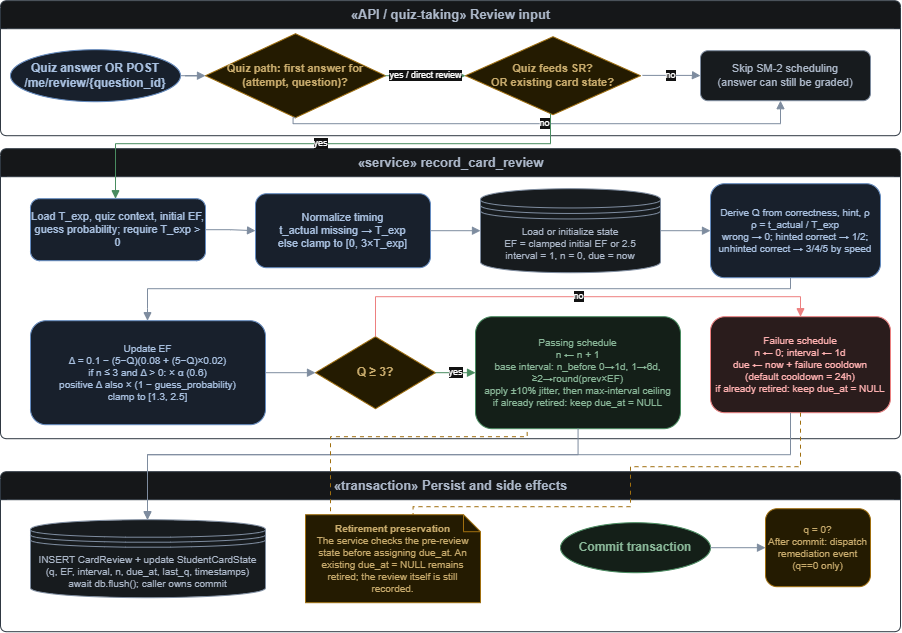
\includegraphics[width=\textwidth]{graphics/act-diagrams/sm2_algorithm_flow.png}
    \caption{SM-2 review scheduling: from graded answer to persisted card state.}
    \label{fig:sm2_algorithm_flow}
\end{figure}


\subsection{Lesson Unlock Gate}
\label{appendix:lesson-unlock-flow}

The gate's three conditions are specified in
Section~\ref{sec:individualised_modeling} and its implementation in
Section~\ref{sec:impl_sr}. Figure~\ref{fig:lesson_unlock_gate} shows what
happens between a learner clicking a lesson and the server deciding whether to
hand over its body.

The diagram exists mainly to make two things unmistakable. The first is that
the verdict is computed on \emph{read} and nowhere else: there is no unlock
event, no service that fires when a threshold is crossed, and no stored
eligibility column --- only a memoised computation and a cache key that writes
invalidate. The second is what the gate does with a malformed prerequisite
graph. The traversal is recursive, so a cycle would not terminate; the
implementation detects one, logs it, and treats the cyclic edge as
\emph{satisfied}. That is a deliberate choice to fail open on a data error the
learner did not cause, and it is the kind of decision a reader will assume is
an oversight unless the diagram shows it as a labelled branch.

Two further details are visible only here. Navigation metadata and lesson
content sit on opposite sides of the boundary --- the curriculum tree tells the
learner a lesson exists and is locked, while every read that would return its
body, its resources, a signed download URL, or its knowledge graph passes
through the gate --- so a locked lesson is discoverable but not readable. And
the whole gate sits behind a single deployment switch, which returns eligible
immediately when set: an escape hatch for the case where a misconfigured
threshold locks a cohort out of its own course mid-term.

\begin{figure}[H]
    \centering
    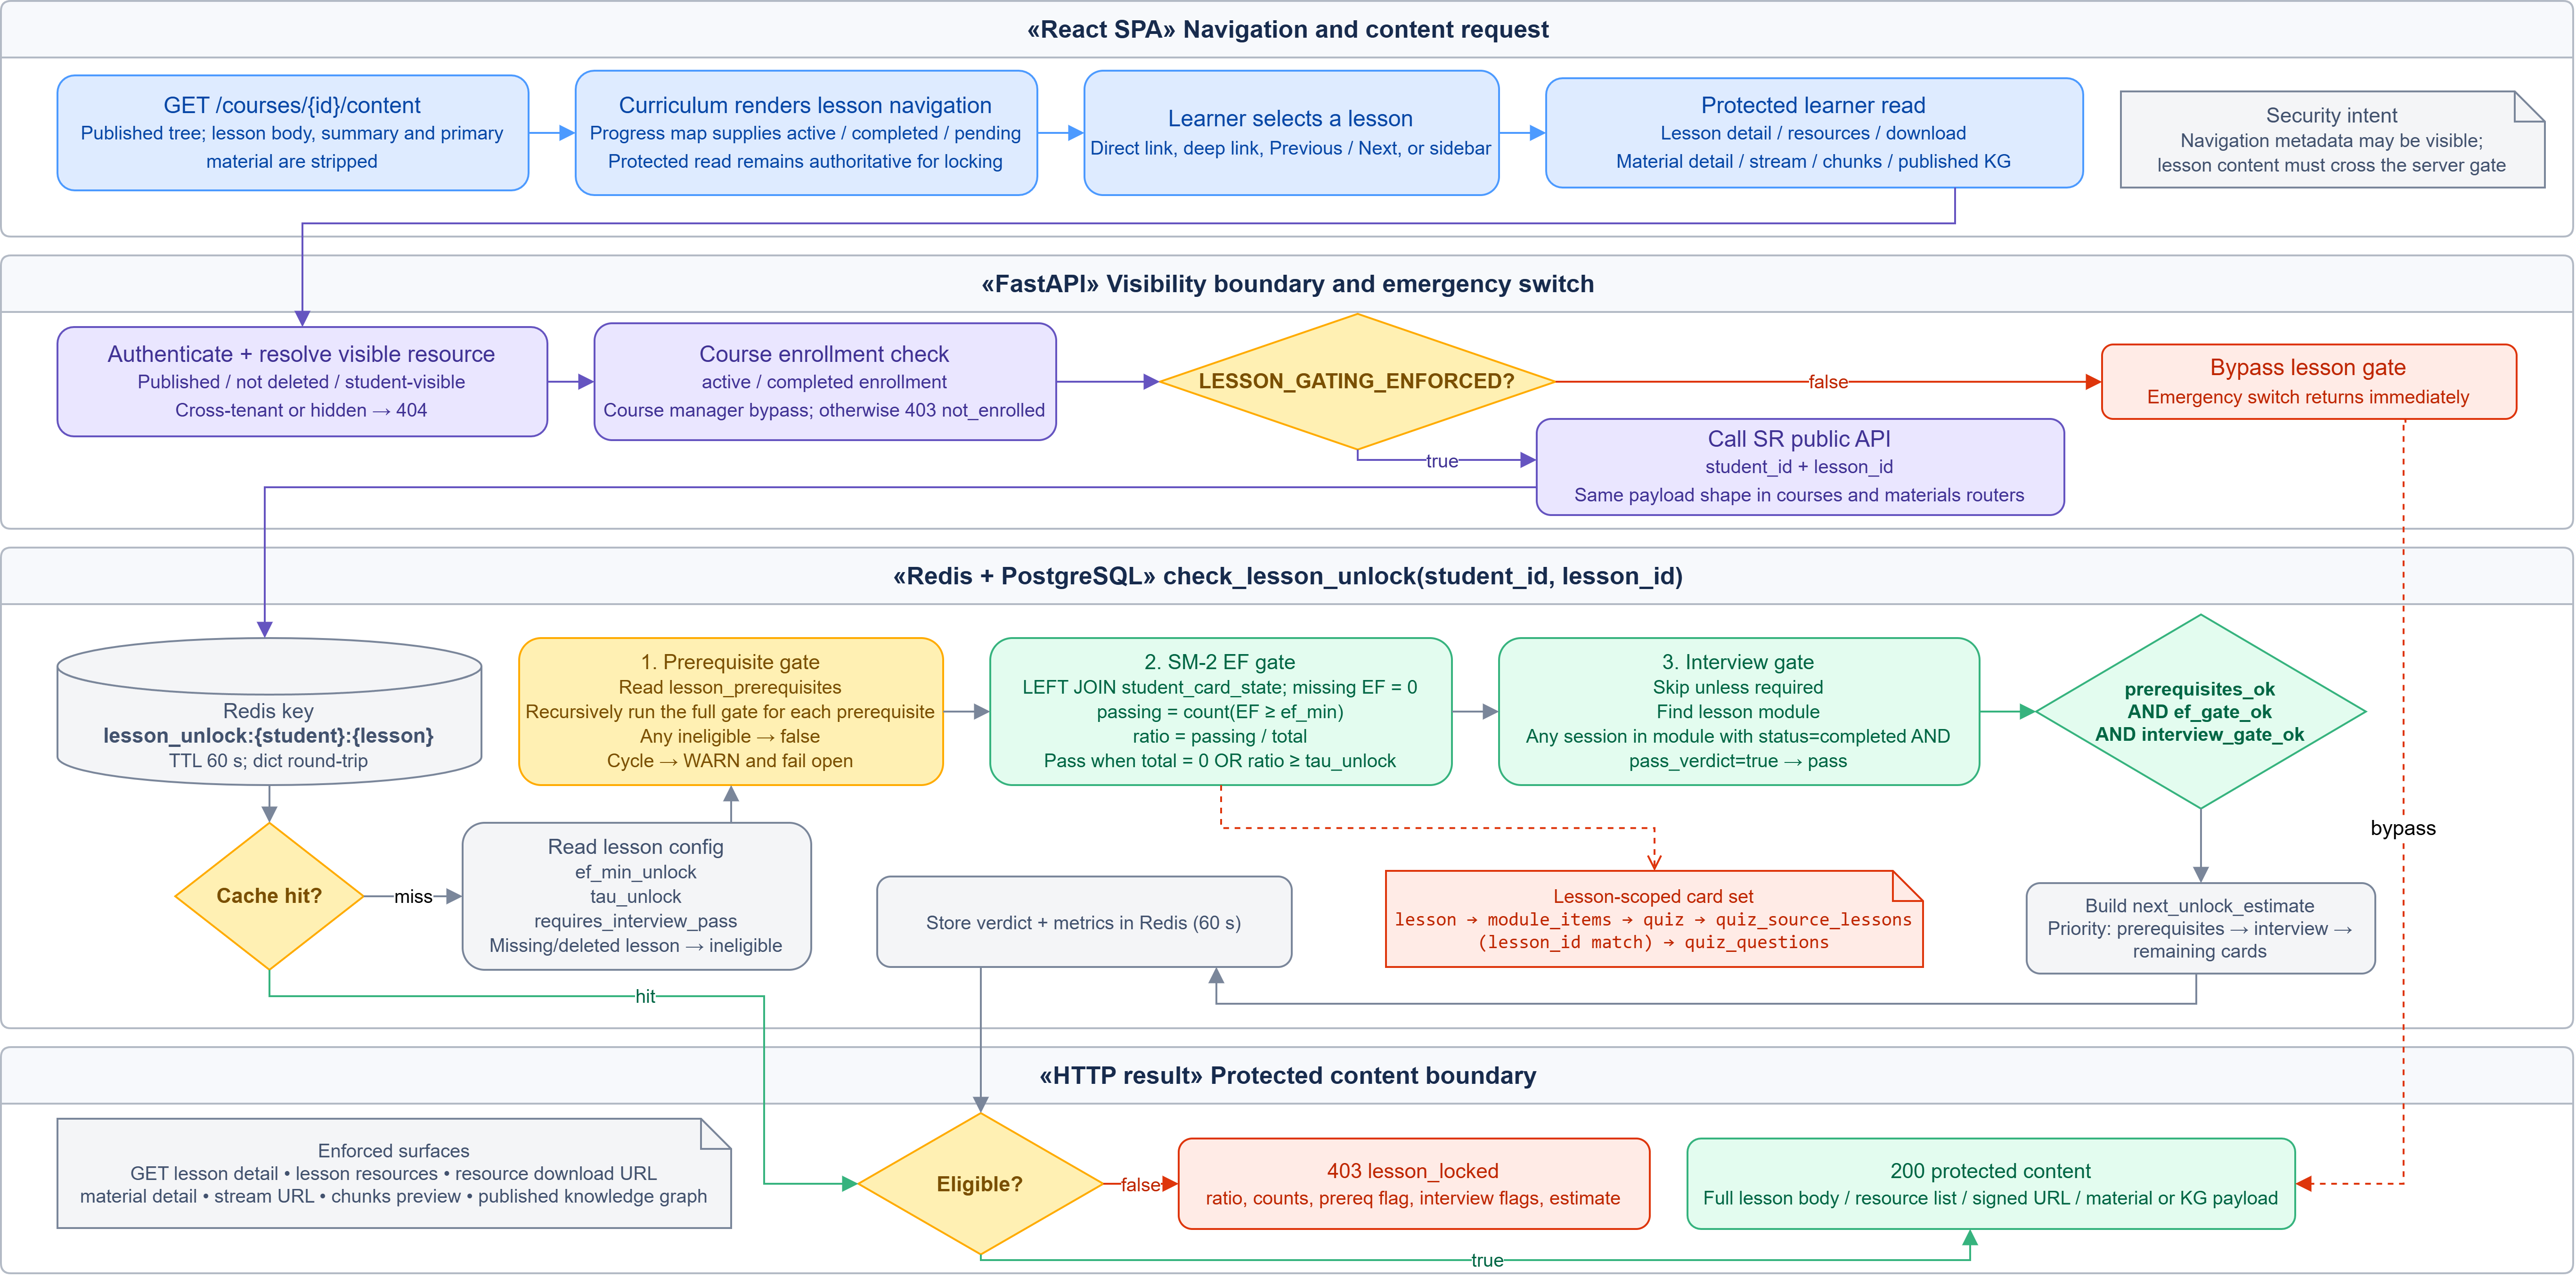
\includegraphics[width=\textwidth]{graphics/act-diagrams/lesson_unlock_gate.png}
    \caption{Lesson unlock gate: enrolment and visibility checks, the three unlock conditions, and the protected-content boundary.}
    \label{fig:lesson_unlock_gate}
\end{figure}

\subsection{Material Ingestion}
\label{appendix:ingestion-flow}

The implementation is described in Section~\ref{sec:impl_ingestion}.
Figure~\ref{fig:material_ingestion_flow} traces one uploaded document from the
teacher's file picker to the knowledge graph a learner eventually reads,
across the three processes that carry it.

Three properties of this flow are the reason it is drawn rather than only
described. The bytes never pass through the API: the browser uploads directly
to object storage against a presigned session, and the API's job afterwards is
to verify that what was promised actually arrived --- which is why a
\texttt{HEAD} check for a phantom or truncated object appears as a rejection
path with no counterpart anywhere else in the system. The work then leaves the
request entirely, so every stage after the enqueue runs in a worker whose
failure is recorded against the material version rather than returned to
anyone. And the last lane is not automatic at all: the AI-extracted graph is a
\emph{seed} for a teacher to curate, publishing is blocked until they do, and
an unavailable graph yields an in-memory placeholder rather than an empty one
--- a distinction with no visible difference until the teacher tries to
publish.

\begin{figure}[H]
    \centering
    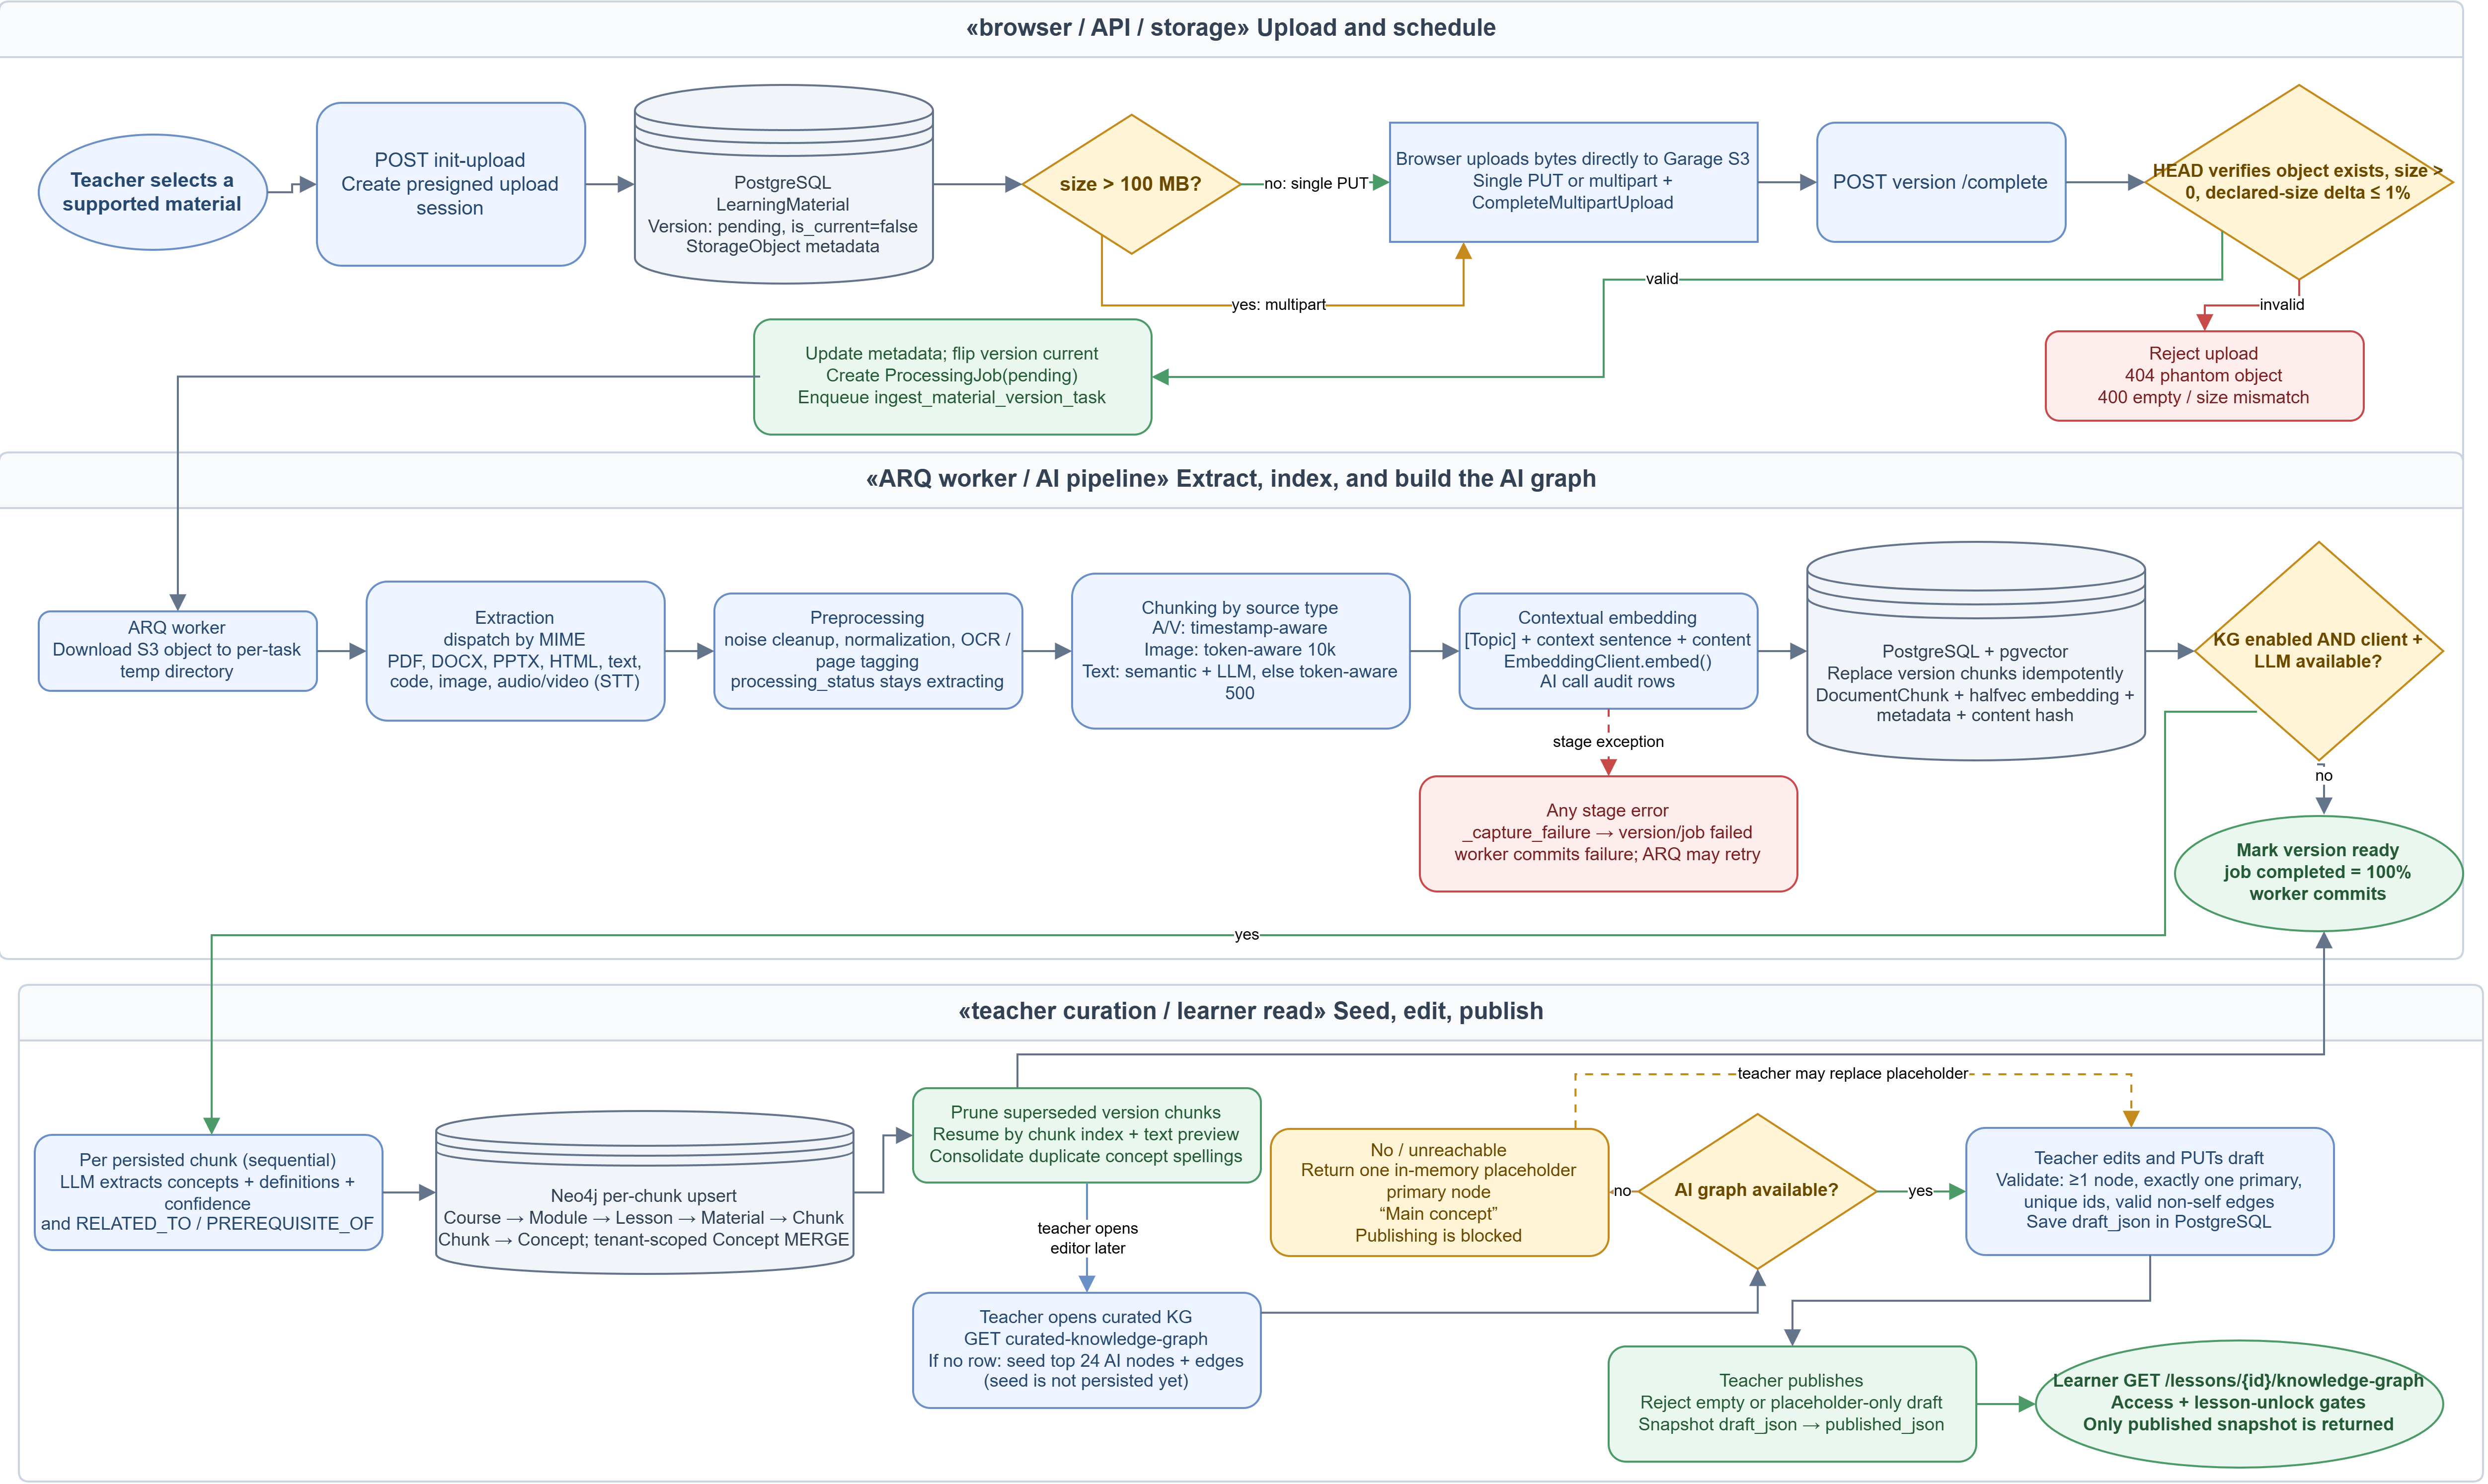
\includegraphics[width=\textwidth]{graphics/act-diagrams/material_ingestion_flow.png}
    \caption{Material ingestion: upload and scheduling, worker extraction and indexing, and teacher curation of the knowledge graph.}
    \label{fig:material_ingestion_flow}
\end{figure}

\subsection{Quiz Generation}
\label{appendix:quiz-generation-flow}

The implementation is described in Section~\ref{sec:impl_quiz_pipeline}.
Figure~\ref{fig:quiz_generation_flow} traces a generation request from the
teacher's click to the questions that land in their review queue.

What the diagram makes visible is that the HTTP request and the work it asks
for are two different things with two different lifetimes. The endpoint
validates, guards, creates a durable run row, enqueues, and returns
\texttt{202} --- at which point the request is over and nothing has been
generated. Everything of substance happens afterwards in a worker, and the
client learns of it only by polling the run it was handed. The consequences of
that split are what the remaining branches encode: a run orphaned by a worker
crash is recovered by a separate sweep rather than by the caller; progress is
checkpointed on its own short-lived database session so a report of progress
survives a pipeline transaction that later rolls back; and the two generation
modes diverge into genuinely different pipelines, topic mode over-generating
to absorb the losses that validation and de-duplication will inflict, coverage
mode budgeting per outline section before it generates anything at all.

\begin{figure}[H]
    \centering
    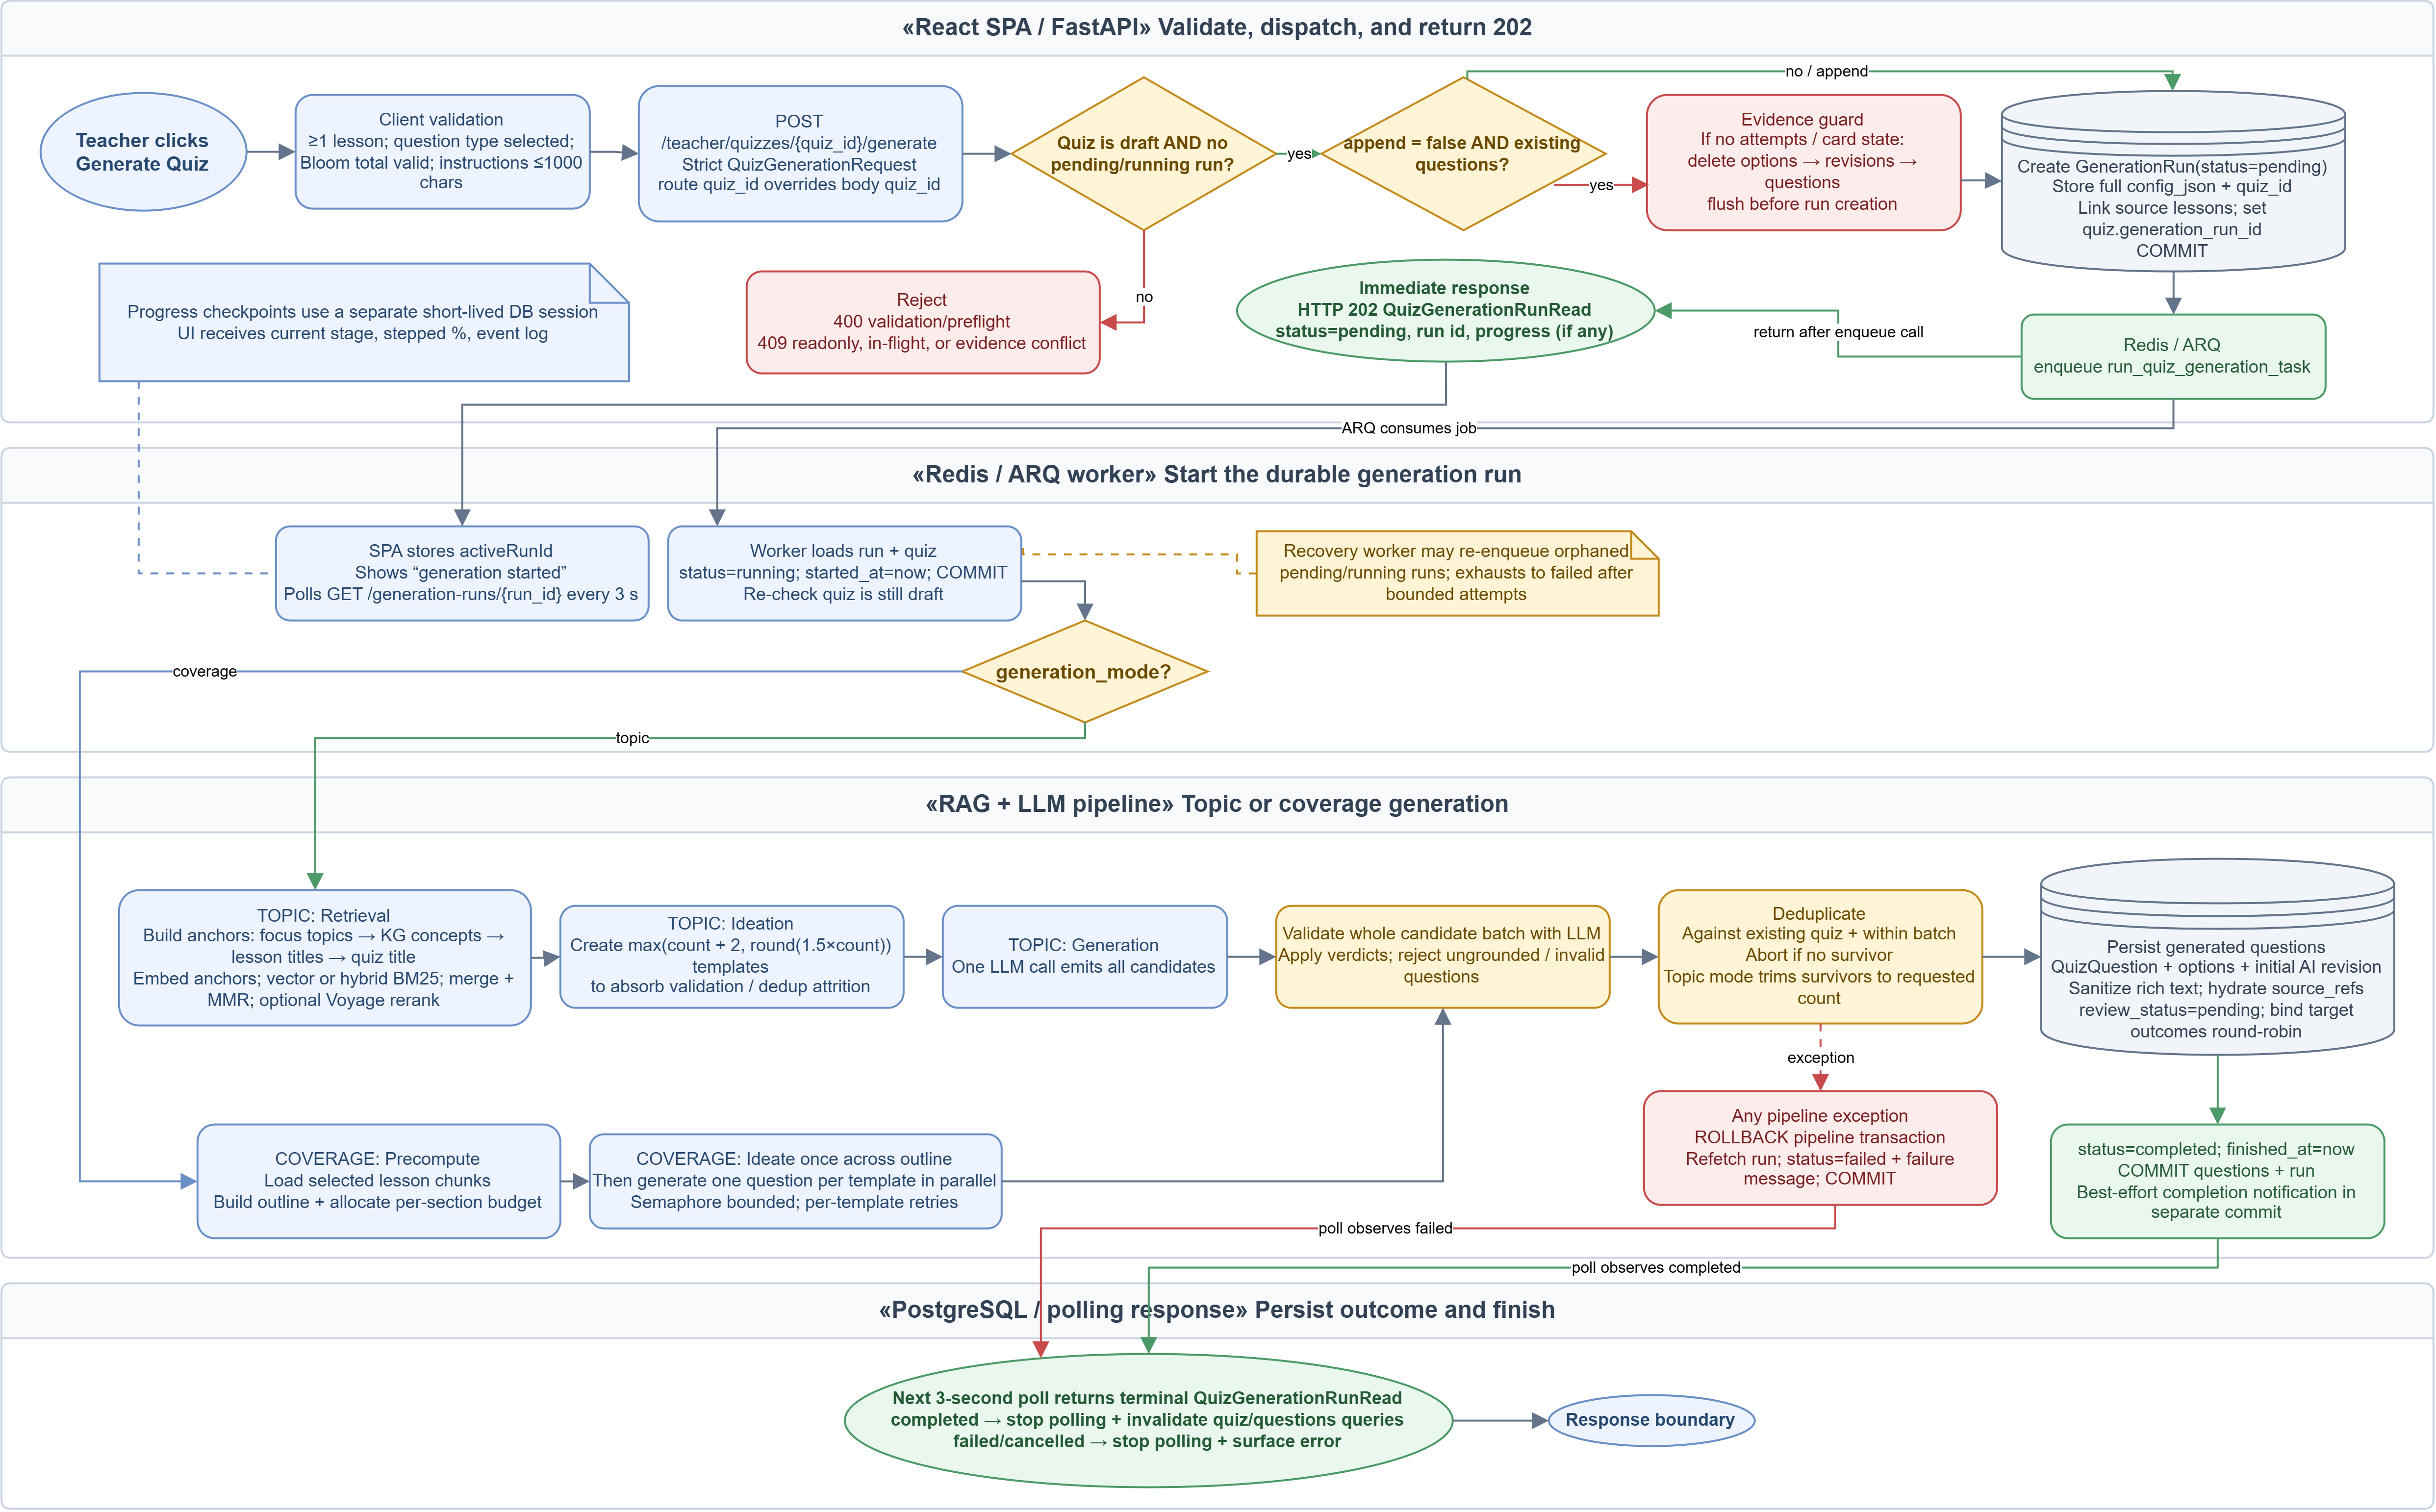
\includegraphics[width=\textwidth]{graphics/act-diagrams/quiz_generation_flow.png}
    \caption{Quiz generation: synchronous validation and dispatch, the durable generation run, the topic and coverage pipelines, and the terminal poll.}
    \label{fig:quiz_generation_flow}
\end{figure}

\subsection{Quiz Attempt Lifecycle}
\label{appendix:quiz-attempt-flow}

The implementation is described in Section~\ref{sec:impl_quizzing}.
Figure~\ref{fig:quiz_attempt_lifecycle} follows one attempt from the intro
screen to the result, and it is the longest flow in the system because an
attempt is the one place where assessment integrity, spaced repetition and
crash recovery all bear on the same rows at the same time.

Three of its properties are worth naming before reading it. Everything that
could change beneath a live attempt is \emph{frozen at creation}: the question
order and option shuffle, the timing, and the integrity policy are all
snapshotted onto the attempt row, so editing the quiz mid-attempt cannot alter
what the student is being measured against. Ownership is a lease rather than a
check --- a Redis entry claimed before the database commit and renewed by
heartbeat --- which is what makes an explicit takeover on a second device
possible without two tabs writing to one attempt. And the SM-2 review fires on
the \emph{first} saved answer to each question only: a later edit still changes
the score, because the answer row is upserted, but it does not reschedule the
card, or a student could tune their own review queue by toggling answers.

The diagram also carries the paths that exist only for things going wrong. An
attempt left open past its deadline is closed by a cron sweep rather than by
the student, and the sweep chooses between submitting it and expiring it
according to the quiz's own policy. A submit flushes every unsaved answer
first and aborts if any of those writes fails, rather than finalising a partial
record. What the result exposes is itself gated: a quiz needing manual grading
returns no score at all, and the visibility policy decides separately whether
the student may see their score, their correctness, or the answers.

\begin{figure}[H]
    \centering
    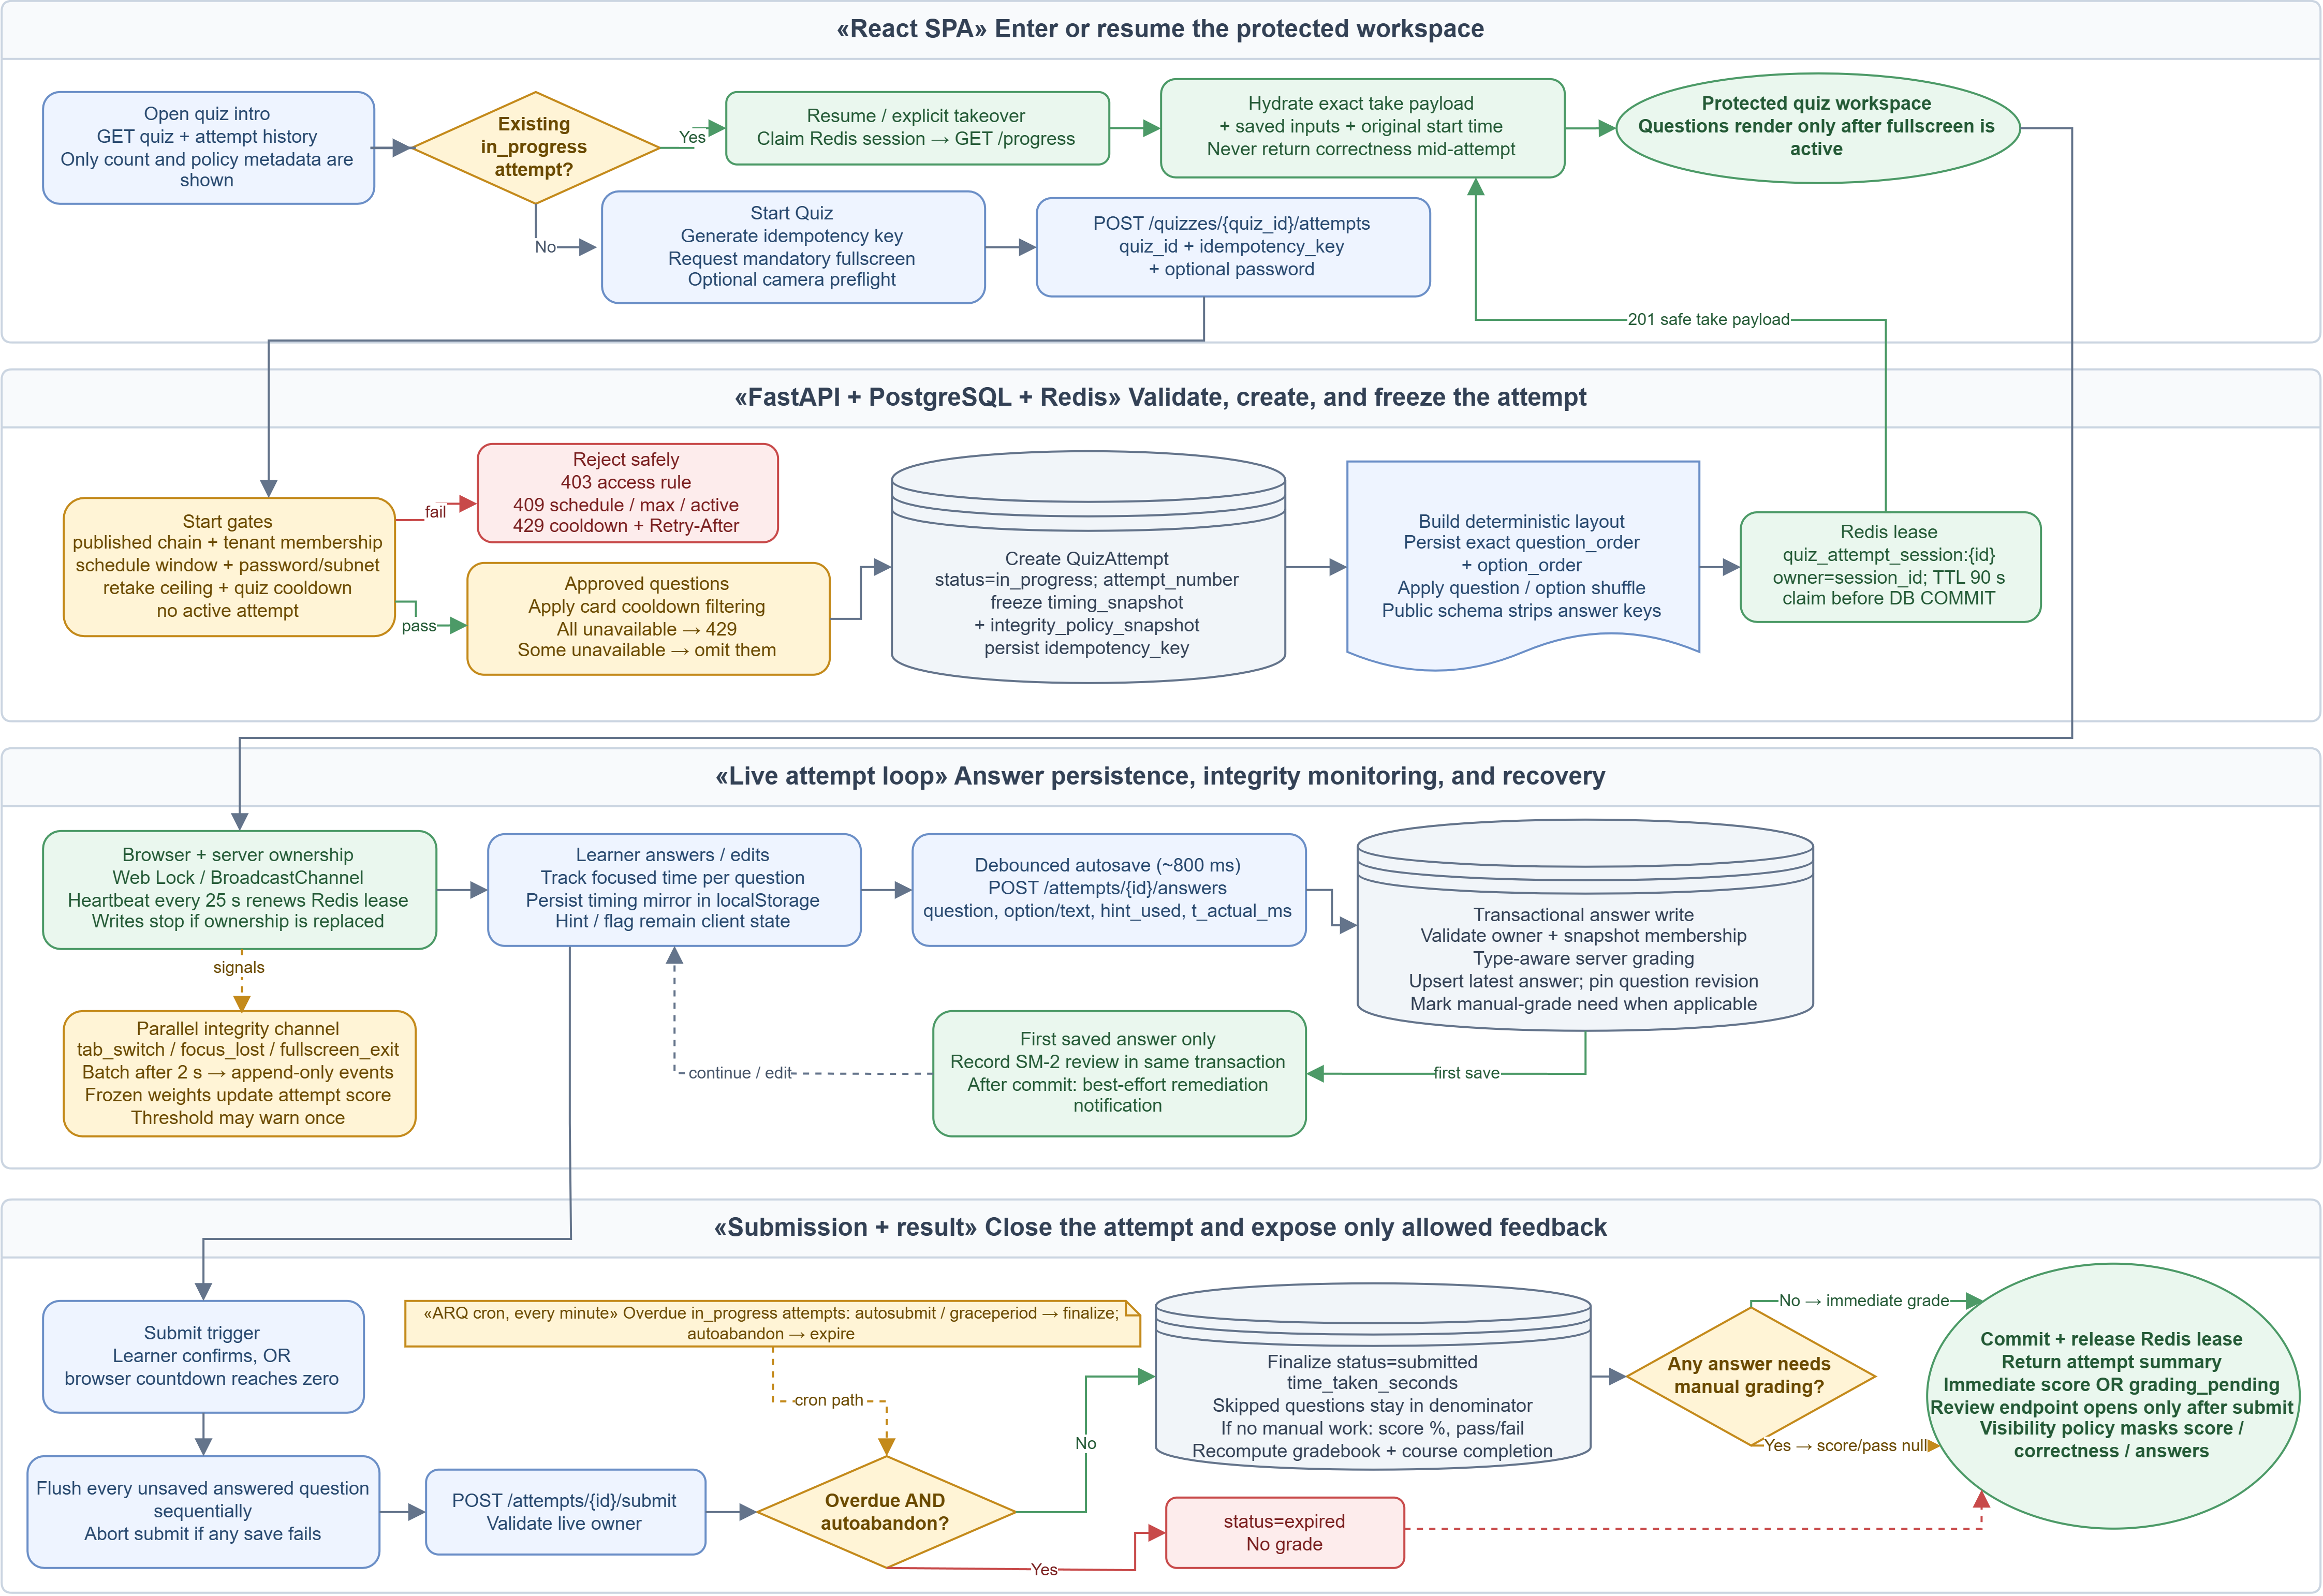
\includegraphics[width=\textwidth]{graphics/act-diagrams/quiz_attempt_life_cycle.png}
    \caption{Quiz attempt lifecycle: entry and resumption, attempt creation and freezing, the live answer loop with integrity monitoring, and submission.}
    \label{fig:quiz_attempt_lifecycle}
\end{figure}

\subsection{Career Pathway Stage Evaluation}
\label{appendix:stage-evaluation}

The rules this evaluator applies are specified in
Section~\ref{sec:pathway_completion}. Figure~\ref{fig:stage_evaluation_flow}
shows the order in which it applies them for one student against one pinned
pathway version: stages are walked in position order, each one's required and
quota-limited elective counts are resolved into a live completion, a latched
completion already recorded is honoured over a live one that has since lapsed,
and the unlock verdict for each stage reads the stage before it --- which is
why the pass runs forward and only once.

\begin{figure}[H]
    \centering
    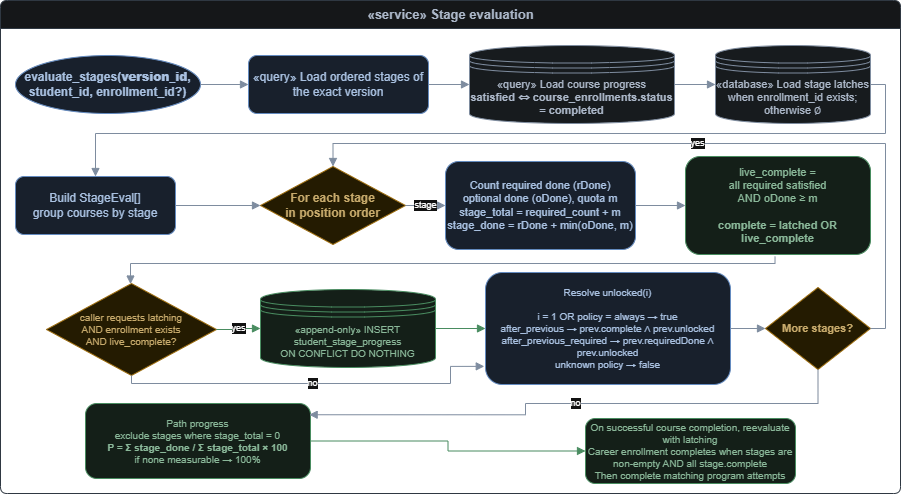
\includegraphics[width=\textwidth]{graphics/act-diagrams/stage_evaluation_flow.png}
    \caption{Career pathway stage evaluation: from pinned version to per-stage completion, unlock, and overall progress.}
    \label{fig:stage_evaluation_flow}
\end{figure}

\subsection{Path Change and Attempt Closure}
\label{appendix:path-change-flow}

The governance model is described in Section~\ref{sec:impl_path_governance}.
Figure~\ref{fig:path_change_attempt_closure} traces a student's request to
switch or drop a career path from creation through a dean's decision to the
downstream access that decision revokes.

This flow is drawn because approving a request is not a status update. The
approval runs inside one transaction that closes the source attempt, writes an
immutable \texttt{exit\_snapshot} of the progress it had earned, creates the
replacement attempt pinned to the target version, and then reconciles every
entitlement the old path had granted. That reconciliation is where the
subtlety lies: grants are transferred only for courses the two paths share and
revoked otherwise, a course enrolment is dropped only when no other live
entitlement still covers it, and completed enrolments and their awards are
preserved regardless. A student who switches paths therefore keeps what they
finished, keeps access to what both paths need, and loses only what the old
path alone justified.

The guards are also checked twice, at different times and for different
reasons. Creation checks that the request is coherent; approval re-checks the
same invariants against the state as it stands at the moment of decision,
because a target path can be archived, or a budget exhausted, between the
request and the review. A change request whose target has since disappeared is
invalidated rather than approved, and no attempt is closed --- the one outcome
that must never be reached by default, since closure is irreversible and the
snapshot it writes is the only record of what the student had earned.

\begin{figure}[H]
    \centering
    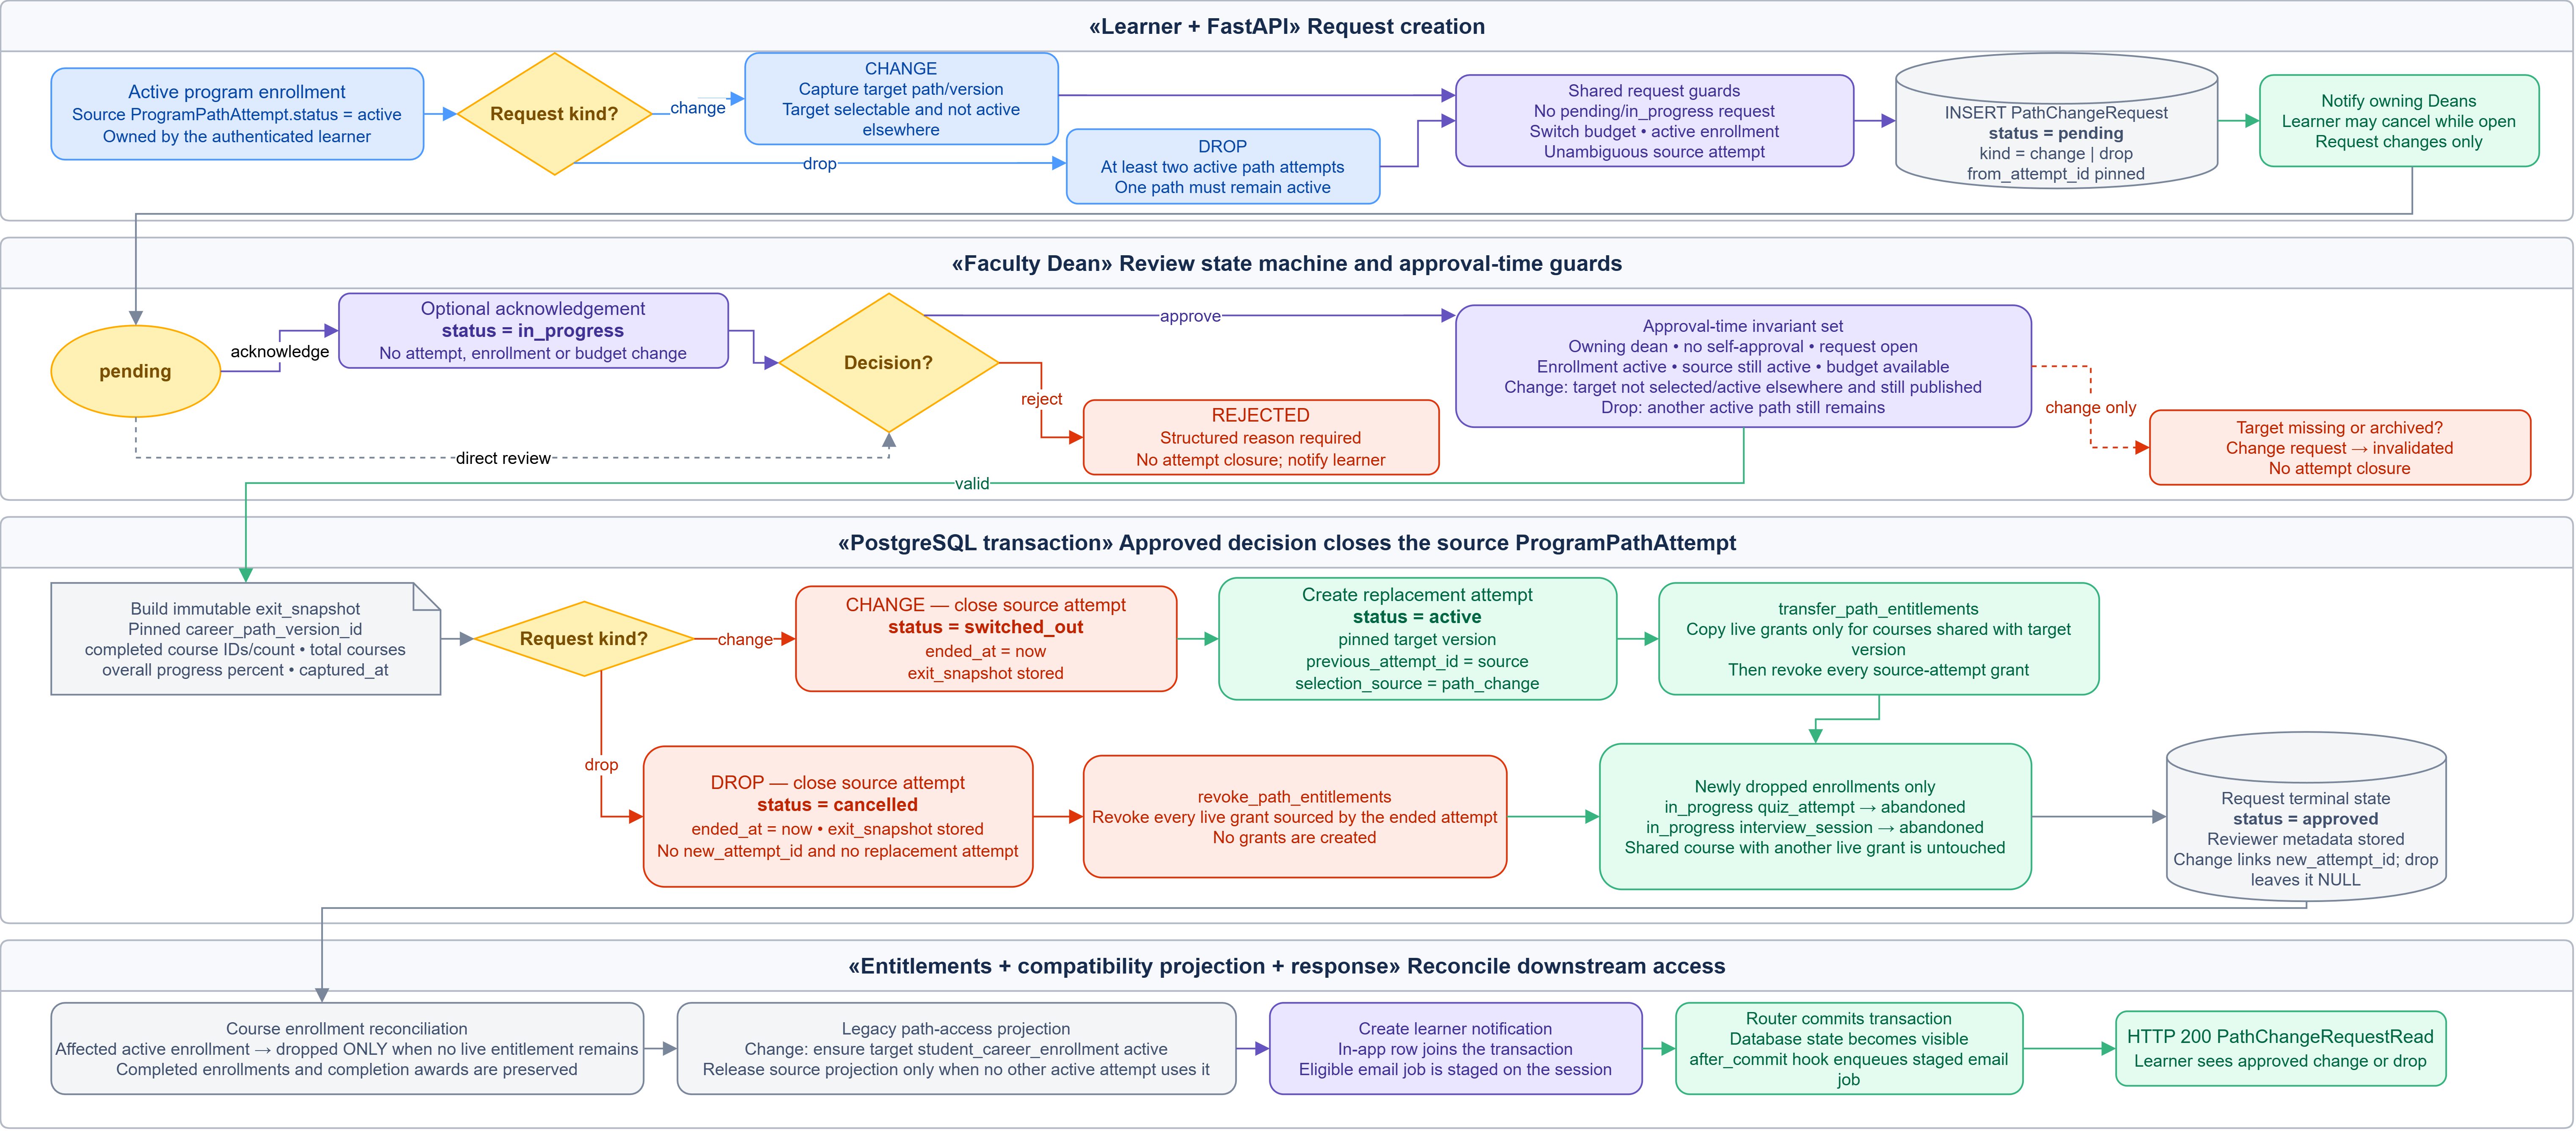
\includegraphics[width=\textwidth]{graphics/act-diagrams/path_change_attempt_closure.png}
    \caption{Path change and attempt closure: request creation, the dean's review state machine, the approval transaction, and downstream entitlement reconciliation.}
    \label{fig:path_change_attempt_closure}
\end{figure}
